%\documentclass[11pt,twocolumn]{article}

\usepackage{mystyle}

\title{Airplane Seating Problem}
\author{James Zuber}
\date{\today}

\begin{document}

\maketitle

\begin{abstract}
We imagine passengers on an airplane being asked to swap seats so that a couple or family can sit together.  This paper focuses on minimizing the number of passenger exchanges to make all families on a plane happy.  We give a hardness proof for the general case of unbounded, heterogeneous family sizes and constant factor approximation heuristics for smaller families on idealized planes.
\end{abstract}

\section{Introduction}
Though passengers on an airplane book their seats as families, we imagine that during boarding many of these families wind up scattered throughout the plane rather than next to each other.  Since the only way to fix this situation without reboarding is single passenger exchanges (swaps), we would like to find the smallest number of swaps necessary so that all families are happily seated together.

\subsection{Prior and Related Work}

Ths problem is closely related to the Dutch Flag problem posed by Djikstra \cite{dijkstra1976discipline}, where a number of colored marbles need to be rearranged from a random order to a final, known configuration.  The correct solutions posed by Djikstra and Meyer were analyzed and found non-optimal by McMaster \cite{mcMaster1978analysis}.  A generalization to any number of colors was proposed and solved optimally \cite{bitner1982asymptotically} using a scanning algorithm with insights that helped us form ours.  This generalization was later named the American Flag problem and shown to have applications for speeding up Radix sorting \cite{mcllroy1993engineering}, \cite{al2005formulation}.

Another related problem is found in kidney exchanges and other market clearinghouses where a number of patient-donor pairs that aren't compatible require trades with other patient-donor pairs for compatible organs.  Market clearinghouses work like our 1D airplanes with large families that only need to seat together in pairs.  The problem is solved by finding a cycle cover of a graph, which was proven NP complete \cite{abraham2007clearing}.  Its impact on saving lives was both simulated \cite{roth2004kidney} and implemented \cite{abraham2007clearing}.  It was also proven that at allowing only 4 pairs of patients in any exchange chain is sufficient to guarantee an optimal cycle cover \cite{roth2007efficient}.

Cycle covers of graphs also find an application in genetics.  This NP complete family of problems \cite{bryant1998complexity}, \cite{durrett2005genomic}, \cite{goldberg2001complexity}, \cite{caprara1999formulations}, \cite{sankoff1997median}, \cite{popov2007multiple} seeks the series of changes in DNA that lead from the DNA sequence of a common ancestor to two (or more) descendents.  Because the mutations and exchanges in DNA over time are functionally identical to swapping passengers, we can reformulate this as a constained seating rearrangement with known starting and ending poisitions.

\subsection{Airplane as a Line Simplification}

Instead of using actual airplane seating charts, we first consider the one dimensional case, where we think of the airplane seats to be arranged in a line, as shown below in figure \ref{fig:lineplane}.  All seats labeled ``A'' are initially populated with a member of the A family, ``B'' the B family, and ``C'' the C family.  You'll note from the figure that we don't care about the ordering within a family (i.e. Dad in seat 1 and Mom in seat 2 is exactly as optimal as Mom in seat 1 and Dad in seat 2). 

\begin{figure}[H]
\label{fig:lineplane}
\centering
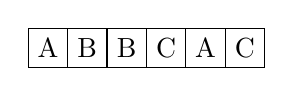
\begin{tikzpicture}[scale=1]
\draw (0,0.0) +(-.25,-.25) rectangle ++(.25,.25);
\draw (0,0.0) node{A};
\draw (0.5,0) +(-.25,-.25) rectangle ++(.25,.25);
\draw (0.5,0) node{B};
\draw (1.0,0) +(-.25,-.25) rectangle ++(.25,.25);
\draw (1.0,0) node{B};
\draw (1.5,0) +(-.25,-.25) rectangle ++(.25,.25);
\draw (1.5,0) node{C};
\draw (2.0,0) +(-.25,-.25) rectangle ++(.25,.25);
\draw (2.0,0) node{A};
\draw (2.5,0) +(-.25,-.25) rectangle ++(.25,.25);
\draw (2.5,0) node{C};
\end{tikzpicture}
\caption{Viewing an airplane as a a line of passengers.}
\end{figure}

In order to make all passengers happy in the smallest number of swaps, we first exchange seats 2 and 5 (which keeps the total number of happy families constant):

\begin{figure}[H]
\centering
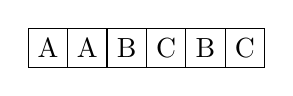
\begin{tikzpicture}[scale=1]
\draw (0,0.0) +(-.25,-.25) rectangle ++(.25,.25);
\draw (0,0.0) node{A};
\draw (0.5,0) +(-.25,-.25) rectangle ++(.25,.25);
\draw (0.5,0) node{A};
\draw (1.0,0) +(-.25,-.25) rectangle ++(.25,.25);
\draw (1.0,0) node{B};
\draw (1.5,0) +(-.25,-.25) rectangle ++(.25,.25);
\draw (1.5,0) node{C};
\draw (2.0,0) +(-.25,-.25) rectangle ++(.25,.25);
\draw (2.0,0) node{B};
\draw (2.5,0) +(-.25,-.25) rectangle ++(.25,.25);
\draw (2.5,0) node{C};
\end{tikzpicture}
\end{figure}

Then we exchange the passengers in seats 3 and 6:

\begin{figure}[H]
\centering
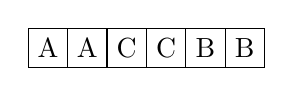
\begin{tikzpicture}[scale=1]
\draw (0,0.0) +(-.25,-.25) rectangle ++(.25,.25);
\draw (0,0.0) node{A};
\draw (0.5,0) +(-.25,-.25) rectangle ++(.25,.25);
\draw (0.5,0) node{A};
\draw (1.0,0) +(-.25,-.25) rectangle ++(.25,.25);
\draw (1.0,0) node{C};
\draw (1.5,0) +(-.25,-.25) rectangle ++(.25,.25);
\draw (1.5,0) node{C};
\draw (2.0,0) +(-.25,-.25) rectangle ++(.25,.25);
\draw (2.0,0) node{B};
\draw (2.5,0) +(-.25,-.25) rectangle ++(.25,.25);
\draw (2.5,0) node{B};
\end{tikzpicture}
\end{figure}

This second swap made 2 families happy with a single swap, and now all families are seated together. Please note that the family blocks are not in alphbetical order, and that any arrangement where all family membes are seated adjacent to each other is optimal.  

Also note that while this required only 2 swaps (the lowest possible for this input) that both swaps involved member of the ``B'' family.  Its possible to generate a pathological case where every swap involves the same passenger yet still minimizes the total number of swaps.  While this does not accurately reflect how grumpy this would make a passenger on our plane, our current model only cares about total number of swaps, future work will limit the maximum number of times a single passenger will have to swap.

\subsection{Limited Family Size Simplification}

While the general case allows passengers to fly together in arbitrarially large, heterogeneous groups, finding the optimal number of swaps in that case is NP-complete (see section \ref{sec:hardness}).  Because of this, we simplify the number of people who can belong to a family in two ways: either we limit the maximum family size in a heterogeneous assortment of families, or we demand all families be the same size.  

\section{Hardness} \label{sec:hardness}

For any case of the known NP-complete problem, 3 partition, there exists an initial passenger location assignment and family size combination where finding the minimum number of swaps possible would mean solving the 3-partition problem.  The reduction follows.

The 3-partition problem is defined as: Given a set of $n = 3m$ integers $x_i$, is there a grouping of the $x_i$ into $m$ disjoint triplets so that the sum of each triplet is the same number $k$?

For any 3-partition instance, we can design the seating arrangement as follows.  There are $m$ blocking families, $B_1, B_2... B_m$ all with the very large number of family members, $M_b > mk$.  For each $x_i$ there is a single family with $x_i$ family members, call these families $f_i$.  Finally there is a single huge family, the Seatwarmers, of size $\sum_i x_i = mk$, that we label $S$.

Our initial seating arrangement is to sit exactly $k$ seatwarmers in the first seats, followed by every member of $B_1$, then alternate between placing a block of $k$ seatwarmers and family $B_i$ until we seat $B_m$ and all $mk$ seatwarmers.  After this we seat all remaining passengers in perfectly rifled order, i.e. $f_1 f_2 f_3 f_1 f_2 f_3 \hdots$.  We sketch this arrangement below (with k = 4, M=2):

\begin{figure}[H]
\centering
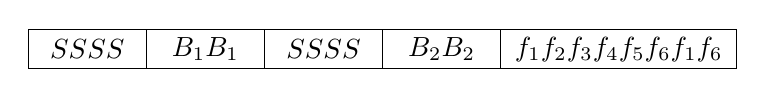
\begin{tikzpicture}[scale=1]
\draw (0,0.0) +(-.75,-.25) rectangle ++(.75,.25);
\draw (0,0.0) node{$SSSS$};
\draw (1.5,0) +(-.75,-.25) rectangle ++(.75,.25);
\draw (1.5,0) node{$B_1 \hdots B_1$};
\draw (3,0) +(-.75,-.25) rectangle ++(.75,.25);
\draw (3,0) node{$SSSS$};
\draw (4.5,0) +(-.75,-.25) rectangle ++(.75,.25);
\draw (4.5,0) node{$B_2 \hdots B_2$};
\draw (6.75,0) +(-1.5,-.25) rectangle ++(1.5,.25);
\draw (6.75,0) node{$f_1 f_2 f_3 f_4 f_5 f_6 f_1 f_6$};
\end{tikzpicture}
\end{figure}
\FloatBarrier

If this problem has a 3 partition, then in exactly $mk$ swaps we can make every family happy by swapping all of the seatwarmers in to the back of the plane, leaving the blocking families in place and in between each set of blocking families putting exactly 3 full $f_i$ families.  

Our toy instance's optimal seating arrangement is:

\begin{figure}[H]
\centering
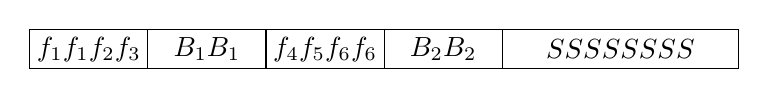
\begin{tikzpicture}[scale=1]
\draw (0,0.0) +(-.75,-.25) rectangle ++(.75,.25);
\draw (0,0.0) node{$f_1 f_1 f_2 f_3$};
\draw (1.5,0) +(-.75,-.25) rectangle ++(.75,.25);
\draw (1.5,0) node{$B_1 \hdots B_1$};
\draw (3,0) +(-.75,-.25) rectangle ++(.75,.25);
\draw (3,0) node{$f_4 f_5 f_6 f_6$};
\draw (4.5,0) +(-.75,-.25) rectangle ++(.75,.25);
\draw (4.5,0) node{$B_2 \hdots B_2$};
\draw (6.75,0) +(-1.5,-.25) rectangle ++(1.5,.25);
\draw (6.75,0)node{$SSSSSSSS$};
\end{tikzpicture}
\end{figure}

\begin{lem}
$mk$ is the minimum number of required swaps $\forall m > 2$
\end{lem}

\begin{proof}
If the seatwarmers all sit together in the back of the plane, it requires one swap per seatwarmer to get back there, or exactly $mk$ swaps.  

By contradiction, assume the seatwarmers don't sit in the final block in the back of the plane.  This means some members of a blocking family $B_i$ have to move.  As long as $M_B > mk$, there are more blocking members in any family than there are seatwarmers, so at most $k$ seatwarmers don't have to change their seat.  Getting the rest to sit in this unmoving block will require $(m-1)k$ swaps.

However, there are now $(m-1)k$ blocking members sitting in the wrong seats.  Since any exchange either puts 0,1 or 2 people in their optimal location, it takes a minimum of $\frac{(m-1)k}{2}$ exchanges to make these blocking members happy.  So long as $\frac{3(m-1)}{2} >= m$ or $m>=3$, this is no better than the $mk$ swaps we achieved using the initial method.
\end{proof}


\section{Solved Cases}

\subsection{Family size of exactly 2}

\noindent
Let us assume that we only have couples on-board, maybe a plane full of honeymooners headed to a post-nuptial resort. For this case, the following sweeping-line algorithm was proposed:

\begin{algorithm}
\caption{ \texttt{Sweep algorithm for families of size two} }
\label{alg:twoSweep}
  \begin{algorithmic}
\While{ $i \leq n-2$ }
  \State Read a pair ($i$, $i+1$) 
  \If{ $couple(i) \neq couple(i+1)$}
   \State let $j = i+2$
   \While{ $couple(j) \ne couple(i)$}
      $j = j + 1$
   \EndWhile
   \State Swap (j, i+1)
  \EndIf
\EndWhile
\caption{ \texttt{Sweep algorithm for families of size two} }
\end{algorithmic}
\end{algorithm}
\FloatBarrier

\begin{thm} \label{thm:sweepCorrectness}
There exists an optimal set of single passenger exchanges where the leftmost position of passengers involved in each exchange is non-decreasing.
\end{thm}


If we imagine a solution to this problem as an ordered pair of seat numbers to be exchanged, $(i_1,j_1), (i_2,j_2)...$ then the following observation can be made. 

\begin{lem} \label{lem:swapRules} 
We can change the order of exchanges using the three rules (with $a,b,c,d$ being unique seat numbers) without changing the final permutation achieved by performing these swaps.

\begin{eqnarray*}
(a,b) (c,d) \rightarrow (c,d) (a,b) \\
(a,b) (a,c) \rightarrow (a,c) (c,b) \\
(a,b) (b,c) \rightarrow (b,c) (a,c) \\
(a,b) (c,a) \rightarrow (c,a) (c,b) \\
\end{eqnarray*}
\end{lem}

\begin{proof}
Assume an odered pair of exchanges has the two exchanges $(a,b) (c,d)$ occurring in sequence. If either $a=b$ or $c=d$, that exchange does nothing and isn't optimal.  By the commutativity of a single exchange, we can insist that $a<b$ and $c<d$.  If $a=b$ and $c=d$, then these two exchanges do nothing and are also not optimal.  The final two cases are that one element of $(a,b)$ is equal to another from $(c,d)$ or that all 4 elements are unique.

When all four elements are unique, performing the first exchange does not change the initial position of either passenger in the second exchange and thus the two exchanges can be completed in any order and preserve exactly the final permutation.

When there is a shared seat being exchanged in both, as in $(a,b) (b,c)$ performing exchange 2 first would change the inhabitant of the repeated seat ($b$) in exchange 1.  Since the previous inhabitant of this seat is now located in the non-shared seat location from the exchange 2, if we want to perform exchange 2 first then we must change exchange 1's shared element ($b$) to the non-shared element of exchange 2 ($c$) in order to perserve the final permuation.
\end{proof}

Proving theorem \ref{thm:sweepCorrectness} is now trivial.

\begin{proof}
If we are given an optimal set of exchanges that are in non-decreasing order of leftmost passenger, we can transform it into a set of exchanges using the same number of swaps that is in non-decreasing order by combining a bubble sort and lemma \ref{lem:swapRules}.

First, we insist that all exchanges be listed with their lowest index first.  Ten we note that in all swaps where an exchange is modified by the rules of lemma \ref{lem:swapRules}, even after making the modifications, the modified exchange will never have a first index smaller than that of the exchange that we just swapped it for.

Finally, starting at exchanges $n-1$ and $n$, we swap the exchanges if the first index of exchange $n$ is lower than that of the exchange $n-1$, and then move on to comparing exchanges $n-1$ and $n-2$.  After one pass, the exchange with lowest left passenger would be our first element. After $n$ passes, the list will be sorted.
\end{proof}

We have only proven that there exists a left to right sweep algorithm that will allow us to seat all couples together, not that our specific sweep algorithm is optimal.  To bridge this gap, we need to make the following observations.

First, because the plane is full of couples, each pair of aligned adjacent seats (where aligned means the first is an odd numbered seat and the second an even numbered seat) will hold a matched couple in the final arrangement.  Any pair of seats in the initial seating arrangement that is not occupied by a matched couple will require at least one exchange to remedy that.

Second, any sweep algorithm will start with the leftmost aligned pair of seats containing a mismatched couple and swap one of those two inhabitants with another passenger in the plane.  Once we prove below that all exchange choices leave the plane in a state that requires the same number of swaps, we can claim that our sweep algorithm is optimal.

\begin{lem} \label{lem:identicalToRelabel}
All exchanges that make one couple happy are equivalent up to a relabeling.
\end{lem}

\begin{proof}
If the first two passengers are parts of the $A$ and $B$ couple, their partners are in one of two configurations (where we only show seats occupied by one member of the $A$ or $B$ couple):
\begin{figure}[H]
\centering
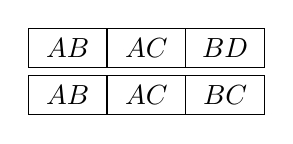
\begin{tikzpicture}[scale=1]
\draw (0,0.0) +(-.5,-.25) rectangle ++(.5,.25);
\draw (0,0.0) node{$A B$};x
\draw (1.0,0) +(-.5,-.25) rectangle ++(.5,.25);
\draw (1.0,0) node{$A C$};
\draw (2.0,0) +(-.5,-.25) rectangle ++(.5,.25);
\draw (2.0,0) node{$B C$};
\draw (0.0,.60) +(-.5,-.25) rectangle ++(.5,.25);
\draw (0.0,.60) node{$A B$};
\draw (1.0,.60) +(-.5,-.25) rectangle ++(.5,.25);
\draw (1.0,.60) node{$A C$};
\draw (2.0,.60) +(-.5,-.25) rectangle ++(.5,.25);
\draw (2.0,.60) node{$B D$};
\end{tikzpicture}
\end{figure}
For the first configuration, we can swap $A$ to be with its partner in either the first or second block:
\begin{figure}[H]
\centering
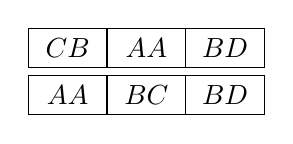
\begin{tikzpicture}[scale=1]
\draw (0,0.0) +(-.5,-.25) rectangle ++(.5,.25);
\draw (0,0.0) node{$A A$};
\draw (1.0,0) +(-.5,-.25) rectangle ++(.5,.25);
\draw (1.0,0) node{$B C$};
\draw (2.0,0) +(-.5,-.25) rectangle ++(.5,.25);
\draw (2.0,0) node{$B D$};
\draw (0.0,.60) +(-.5,-.25) rectangle ++(.5,.25);
\draw (0.0,.60) node{$C B$};
\draw (1.0,.60) +(-.5,-.25) rectangle ++(.5,.25);
\draw (1.0,.60) node{$A A$};
\draw (2.0,.60) +(-.5,-.25) rectangle ++(.5,.25);
\draw (2.0,.60) node{$B D$};
\end{tikzpicture}
\end{figure}
Other than changing which pair of seats are occupied, we have a happy couple $A$ and two pairs of unhappy patrons, $BC$ and $BD$.  These configurations require the exact same number of swaps to rectify.

If we instead swapped $B$, we'd get two configurations also:
\begin{figure}[H]
\centering
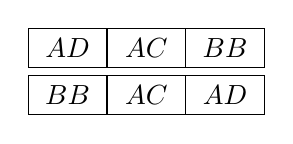
\begin{tikzpicture}[scale=1]
\draw (0,0.0) +(-.5,-.25) rectangle ++(.5,.25);
\draw (0,0.0) node{$B B$};
\draw (1.0,0) +(-.5,-.25) rectangle ++(.5,.25);
\draw (1.0,0) node{$A C$};
\draw (2.0,0) +(-.5,-.25) rectangle ++(.5,.25);
\draw (2.0,0) node{$A D$};
\draw (0.0,.60) +(-.5,-.25) rectangle ++(.5,.25);
\draw (0.0,.60) node{$A D$};
\draw (1.0,.60) +(-.5,-.25) rectangle ++(.5,.25);
\draw (1.0,.60) node{$A C$};
\draw (2.0,.60) +(-.5,-.25) rectangle ++(.5,.25);
\draw (2.0,.60) node{$B B$};
\end{tikzpicture}
\end{figure}

These cases are, exactly like the $A$ swapping cases, equivalent in terms of how many swaps would be required to finish pairing the rest of the plane.  The second possible initial case (where $A$ and $B$ are both seated next to family $C$, yields similarly equivalent situations after an exchange for $A$:
\begin{figure}[H]
\centering
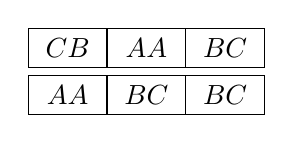
\begin{tikzpicture}[scale=1]
\draw (0,0.0) +(-.5,-.25) rectangle ++(.5,.25);
\draw (0,0.0) node{$A A$};
\draw (1.0,0) +(-.5,-.25) rectangle ++(.5,.25);
\draw (1.0,0) node{$B C$};
\draw (2.0,0) +(-.5,-.25) rectangle ++(.5,.25);
\draw (2.0,0) node{$B C$};
\draw (0.0,.60) +(-.5,-.25) rectangle ++(.5,.25);
\draw (0.0,.60) node{$C B$};
\draw (1.0,.60) +(-.5,-.25) rectangle ++(.5,.25);
\draw (1.0,.60) node{$A A$};
\draw (2.0,.60) +(-.5,-.25) rectangle ++(.5,.25);
\draw (2.0,.60) node{$B C$};
\end{tikzpicture}
\end{figure}

And $B$

\begin{figure}[H]
\centering
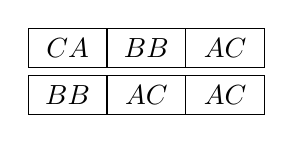
\begin{tikzpicture}[scale=1]
\draw (0,0.0) +(-.5,-.25) rectangle ++(.5,.25);
\draw (0,0.0) node{$B B$};
\draw (1.0,0) +(-.5,-.25) rectangle ++(.5,.25);
\draw (1.0,0) node{$A C$};
\draw (2.0,0) +(-.5,-.25) rectangle ++(.5,.25);
\draw (2.0,0) node{$A C$};
\draw (0.0,.60) +(-.5,-.25) rectangle ++(.5,.25);
\draw (0.0,.60) node{$C A$};
\draw (1.0,.60) +(-.5,-.25) rectangle ++(.5,.25);
\draw (1.0,.60) node{$B B$};
\draw (2.0,.60) +(-.5,-.25) rectangle ++(.5,.25);
\draw (2.0,.60) node{$A C$};
\end{tikzpicture}
\end{figure}

In all cases, exchanging either $A$ or $B$ first left us with conifgurations that were identical up to relabeling $A$ and $B$.  Further, swapping $A$ or $B$ out of the first pair into the seat beside its partner left us with identical configurations up to a reordering of seats.
\end{proof}

Since all sweep algorithms that make at least one couple happy with every exchange are equivalent, and there exists an optimal sweep algorithm that does exactly that, we have proven that our sweep alorithm finds the lowest number of required exchanges.

\section{Mixed families -- couples and singletons}

Let us now consider the case where we have a mixture of couples and singletons, where we want to seat all of the couples together. We assume that singletons are always happy, regardless of whom they sit next to.

\subsection{Phase One, determining structure:} 

We first observe that the worst case scenario for performing exchanges is when we have a situation like:

\begin{equation*}
eAABBCCDDe
\end{equation*}

This requires 4 swaps, or one swap per couple between the two unhappy members of the $e$ pair.  In terms of defining structure beforehand, this was an example of the following situation (where solid boxes will be occupied by a couple, and dotted by singletons):

\begin{figure}[H]
\centering
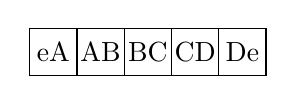
\begin{tikzpicture}[scale=1]
\draw (0.0,0) +(-.3,-.3) rectangle ++(.3,.3);
\draw (0.0,0) node{eA};
\draw (0.6,0) +(-.3,-.3) rectangle ++(.3,.3);
\draw (0.6,0) node{AB};
\draw (1.2,0) +(-.3,-.3) rectangle ++(.3,.3);
\draw (1.2,0) node{BC};
\draw (1.8,0) +(-.3,-.3) rectangle ++(.3,.3);
\draw (1.8,0) node{CD};
\draw (2.4,0) +(-.3,-.3) rectangle ++(.3,.3);
\draw (2.4,0) node{De};
\end{tikzpicture}
\end{figure}

With this assignment, we can clearly see that all passengers are seated in an incorrect seat to start. If instead the two $e$ passengers were singletons, then the following structural assignment would have allowed us to keep all passengers in their starting seats and require zero swaps.

\begin{figure}[H]
\centering
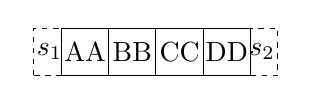
\begin{tikzpicture}[scale=1]
\draw[dash pattern= on 2pt off 2pt] (0,0) +(-.2,-.3) rectangle ++(.15,.3);
\draw (0.0,0) node{$s_1$};
\draw (0.45,0) +(-.3,-.3) rectangle ++(.3,.3);
\draw (0.45,0) node{AA};
\draw (1.05,0) +(-.3,-.3) rectangle ++(.3,.3);
\draw (1.05,0) node{BB};
\draw (1.65,0) +(-.3,-.3) rectangle ++(.3,.3);
\draw (1.65,0) node{CC};
\draw (2.25,0) +(-.3,-.3) rectangle ++(.3,.3);
\draw (2.25,0) node{DD};
\draw[dash pattern= on 2pt off 2pt] (2.7,0) +(-.15,-.3) rectangle ++(.2,.3);
\draw (2.7,0) node{$s_2$};
\end{tikzpicture}
\end{figure}

To properly assign a structure to a seating arangement for singletons and couples that minimizes swaps, we generalize the above bad example.  Sets of paired individuals already seating by their partners are known as blocks.  Our bad example had $AABBCCDD$ all starting in good places, and thus we had a block of $N = 4$ couples.  Our block was out of alignment with our first seating type assignment and would require $N$ swaps to satisfy all seating requirements.  On the other hand, the block was in perfect alignment with the second seating type assignment and required no swaps to be seated.

\begin{figure}[H]
\centering
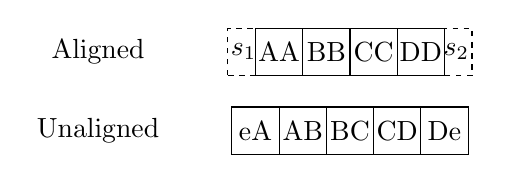
\begin{tikzpicture}[scale=1]
\draw (-2,1) node{Aligned};
\draw[dash pattern= on 2pt off 2pt] (-0.15,1) +(-.2,-.3) rectangle ++(.15,.3);
\draw (-0.15,1) node{$s_1$};
\draw (0.3,1) +(-.3,-.3) rectangle ++(.3,.3);
\draw (0.3,1) node{AA};
\draw (0.9,1) +(-.3,-.3) rectangle ++(.3,.3);
\draw (0.9,1) node{BB};
\draw (1.5,1) +(-.3,-.3) rectangle ++(.3,.3);
\draw (1.5,1) node{CC};
\draw (2.1,1) +(-.3,-.3) rectangle ++(.3,.3);
\draw (2.1,1) node{DD};
\draw[dash pattern= on 2pt off 2pt] (2.55,1) +(-.15,-.3) rectangle ++(.2,.3);
\draw (2.55,1) node{$s_2$};

\draw (-2,0) node{Unaligned};
\draw (0.0,0) +(-.3,-.3) rectangle ++(.3,.3);
\draw (0.0,0) node{eA};
\draw (0.6,0) +(-.3,-.3) rectangle ++(.3,.3);
\draw (0.6,0) node{AB};
\draw (1.2,0) +(-.3,-.3) rectangle ++(.3,.3);
\draw (1.2,0) node{BC};
\draw (1.8,0) +(-.3,-.3) rectangle ++(.3,.3);
\draw (1.8,0) node{CD};
\draw (2.4,0) +(-.3,-.3) rectangle ++(.3,.3);
\draw (2.4,0) node{De};
\end{tikzpicture}
\end{figure}

To fully represent a starting seating arrangement, we must note which passengers are not in blocks, contigious seats thus occupied will be called gaps.  While all blocks will be of even length (because they're comprised of couples), gaps can be of even or odd length.  I will refer to the parity of a gap as odd or even depending on whether the number of elements in it are odd or even.

\begin{lem} \label{lemma:ParityOnly}
For each starting block of size $N_i$, the optimal structural assignment will have a contiguous block of $N_i$ coupled seats. These can either be at the starting location or offset from that position by 1.
\end{lem}

\begin{proof}[Proof that contiguous blocks remainin in place.]
By contradiction.  Let's suppose that the first (left) $k$ couples are declared to be aligned improperly with seats asigned to couples, and the remaining $N-k$ to be aligned properly.  In order for this to occur, there had to be a singleton seat at the transition from aligned to unaligned.  

In order for this structural assignment to be optimal, there can't be a place to put this singleton that would require fewer swaps than the middle of this block.  However, placing it to the left of the $k$ unaligned couples would allow them to all be properly aligned, and reduce the number of swaps required by $k$.
\end{proof}

This in hand, we are going to ask how many existing blocks are going to have to be declared unaligned in order to globally minimize the number of swaps we perform. When a block is declared unaligned, we mean that instead of saying its first and second passengers (who are presupposed to be a couple due to this being a block) are in a single pair of couple designated seats, that instead they are siting in two different designated paired seats.  i.e.


We need another lemma before we can get an algorithm out of these observations.

\begin{lem} \label{lem:oddGapsNeedSingletons}
To satisfy all couples in an odd parity gap without disturbing its neighboring blocks, an odd number of singleton seats will be assigned to the gap.
\end{lem}

\begin{proof}
All seats not assigned to a singletons are assigned in pairs to couples.  All assigned couples take up an even number of seats leaving an odd number of seats to fill with singletons.
\end{proof}

\begin{cor}
All odd gaps require at least one singleton seat to be assigned to it.
\end{cor}

\begin{cor}
Any structural assignment with more odd parity gaps than singleton passengers will require that some blocks move.
\end{cor}

So which blocks move?  With $O$ representing a gap of odd parity, $E$ a gap of even parity, and $B$ being a block, the following situations exhaustively describe gap-block borders:

\begin{align*}
O B O \\
E B O \\
O B E \\
E B E \\
O B_1 E B_2 E B_3 \hdots B_k O \\
\end{align*}

In the first situation, if we declare the block unaligned and then perform the $N$ couple swaps to make it a block again, we wind up with $E B E$ and two fewer odd parity gaps.  

If we declare the block unaligned in the second or third cases, and preform $N$ couple swaps to make it a block again, we wind up with $O B E $ and $E B O$ respectively but keep the number of odd parity gaps constant.  The third case would become $O B O$, generating two aditional odd parity gaps.

The final case would become $E B_1 E B_2 E \hdots B_k E$.  This would reduce the number of odd parity gaps by 2 and cost $\sum_{i=1}^k |B_i|$ swaps.  Please note that only shifts between adjacent odd parity gaps decrease the number of odd parity gaps that we have, that all such shifts decrease our number of odd parity gaps by 2 and that they all cost a number of swaps equal to the number of couples in the blocks between them all.

\begin{lem} \label{lem:shiftLeftRightIdentical}
Shifting a block surrounded by odd gaps either to the right or left makes both of its odd parity gap neighbors even, and are equivalent in terms of total swaps left to pair all couples.
\end{lem}

\begin{proof}
The gap reduction part was argued above, so we need only prove equivalence.  A block bordered by two odd gaps has two neighbor passengers, $x$ and $y$.  After moving the block one to the left, we will shift passenger $x$ to the right side of the block, immediately before passenger $y$.  If $x$ and $y$ match, they increase the size of the block, if they don't, we know that $y$ didn't match its right neighbor otherwise it would have been a part of a block rather than an odd gap.

If we move the block to the right, then passenger $y$ winds up one unit to the left of the block next to $x$ again. Since we know that $x$ wasn't partnered with its neighbor to the left, the only new passible partnership is, as before, $x$ and $y$.

Thus moving a block left or right are equivalent in terms of number of swaps left to complete all pairings.
\end{proof}

\subsection{Dynamic Program for Gap Assignment}

A simple dynamic program can answer the question: which blocks do we declare unaligned in the optimal seating structure?  

Diagramatically, we have:

\begin{figure}[H]
\centering
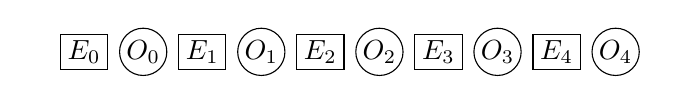
\begin{tikzpicture}[scale=.75]
\draw (-0.3,0) node{$\hdots$};
\foreach \x in {0, 1, 2, 3, 4}
{
  \draw (0.5+2*\x,0) +(-.4,-.3) rectangle ++(.4,.3);
  \draw (0.5+2*\x,0) node{$E_\x$};
  \draw (2*\x+1.8,.3) +(-.3,-.3) circle (.4);
  \draw (2*\x+1.5,0) node{$O_\x$};
}
\draw (10.3,0) node{$\hdots$};
\end{tikzpicture}
\end{figure}

If $E_i$, the block between odd gap $i$ and $i+1$ has $N_i$ paired couples, and we label the number of required swaps to fix parity $S(x,k)$ where $x$ is the index of the block we're moving and $k$ is the number of odd parity gaps we've closed.

Our recurrence relation is: 

\begin{equation*}
  S(x,k) = \min_x S(x-2, k-2) + N_{x}
\end{equation*}

Memoizing this table takes the number of odd gaps times the number of gaps we have to close.  Since each gap has to end with a block, the number of odd gaps is no more than $\frac13$ of our total number of seats.  Since we can't close more gaps than we have, this simple algorithm is, at worst, quadratic in number of passengers.  

\subsection{Performing the Swap Sweep}

After the dynamic program is run, we perform the swaps it indicated.  This leaves us with a set of subproblems, the gaps between blocks (who will not move again).  Even gaps are easier to solve than odd gaps because their parity is already set, so we'll start with them.  While sweeping through a gap, we look at two elements at a time, seats $i$ and $i+1$.  With $s$ representing singletons, and all capital letters representing couple members, there are five distinct cases, each of which get treated differently.

\begin{itemize}
\item $AA$ 
Though it would seem that this shouldn't happen as gaps are filled with unpaired passengers, earlier steps in our sweep algorithm can leave these completed pairings in place.  When enountered, leave them there.
\item $AB$ 
The same arguments from Lemma \ref{lem:identicalToRelabel} hold here and swapping either $A$ or $B$ with its pair elsewhere in the plane leaves the passenger arrangement identical up to a relabeling.  When encountered, swap $B$ for the partner of $A$.
\item $As$
The same arguments from Lemma \ref{lem:identicalToRelabel} hold here with some slight modification. The relabeling would be calling 2 specific singletons $A$.  Since singletons have the potential to be left in place (saving swaps) swapping in the partner to $A$ will always be the optimal answer.  When encountered, exchange $s$ for the partner for $A$.
\item $sA$ 
This case is more complicated, as we can leave the singleton in place if we have 2 more singletons than we have odd parity gaps, and we have a complementary $Bs$ in this same gap.  When encountered, if we have 2 extra singletons in the budget, scan from right of this gap. If there is a matching $Bs$, leave both singletons in place and turn this gap into 2 new gaps: the one between these 2 singletons, and the gap between the right singleton and the next block.  Else, swap the $s$ for the matching $A$.
\item $ss$ 
Leave in place permanently if we have 2 more free singletons than odd parity gaps, temporarially if we are going to have to use these singletons.
\end{itemize}

By Lemma \ref{lem:identicalToRelabel}, and the observation that when an swap is identical up to a relabel, if the singletons are moved to an incomplete portion of the plane, they can never require more swaps than if we instead moved halves of couples.

\begin{lem} \label{lem:splitOddGaps}
Permanently leaving a singleton at an odd position in an odd length gap partitions it into 2 even length gaps that can be scanned using the above rules.
\end{lem}

Following this order, we have 2 types of odd length gaps left: those with singletons in even numbered seats (counting from their first seat) and those with no singletons.  Each of these gaps needs 1 singleton in an odd numbered seat to apply Lemma \ref{lem:splitOddGaps} and then scan using the even gap rules.  To scan odd gaps with singletons in them, we add in one rule:

\begin{itemize}
\item{$As$}
To save a single exchange, if the other $A$ is in an odd seat, exchange the $s$ for that $A$ and then use even scan rules on the 2 even gaps just created.  If the other $A$ is in an even seat, exchange this pair from $As$ to $sA$ and continue this gap as if it were even.
\end{itemize}

With only odd length gaps remaining that have no singletons in them, we need to swap in singletons that were left in their original seats using the $ss$ rule.  While scnaning these gaps, we use the simple rules:

\begin{itemize}
\item{$A_1 B$}
If $A_2$ is also in an odd seat, trade both $A_1$ and $A_2$ for a pair of singletons sitting next to each other in a completed gap. Then complete the 3 newly created even gaps using the even gap rules.
\item{$A_1-$}
When we reach the end of a gap without encountering the previous situation, trade both $A_1$ and $A_2$ for a pair of singletons sitting next to each other in a completed gap. Then scan the gap that previously contained $A_2$.
\end{itemize}

\subsection{Computer Simulations and Results}

In order to verify our hunch that the above algorithm was optimal, we coded up our algorithm in C++ and ran it on a PC. Each passenger was represented by a data structure: all passengers have a family name, a chair number, and know the family name of their left and right neighbors and the location of their partner.  Indices of seats occupied by singletons were stored in a single sorted array to allow range queries of singletons to occur in logarithmic time.

We sought to uncover the worst cases ecountered by our algorithm and devised the following simple test: starting from a completely content plane, we would select and exchange $k$ random passengers.  Because the optimal number of exchanges to return the plane to a completely content state must be no greater than $k$, we could compare the number of exchanges our algorithm found to $k$ in order to find the worst case performance ratio.  Any performance ratio less than 1 was discarded since this meant that the initial shuffling was simple enough that it could be undone in less than $k$ exchanges.

In order to find the high performance ratios, we allowed a genetic algorithm to search the space of shiffled seating arrangements.  For a plane of size $N$ with fixed $N_s \leq N$ singletons, the GA's genes first $N_s$ alleles were the indices of the singletons.  The next $2k$ indices were each interpreted as a pair of passenger positions to swap.  

The initial conifguration routine first sorted the list of singletons, then handled duplicate entries and having an odd number of seats between consecutive singletons. The vacant seats were occupied by content couples.  Finally the swapping portion of the genes were applied and passenger data structures were kept up to date with each swap.

It became almost immediately apparent that our algorithm was not optimal, as even modest sized problems ($N = 100, k = 10$) had worst case performance ratios above 1.6 after a few hundred generations.

\subsection{Win-Win Exchanges, Completed Couples and N-Chains}

Analysis of the genetic algorithm's worst case returns pointed us towards the following conclusion: we weren't handling win-win exchanges properly.  A win-win exchange is of the form:

\begin{figure}[H]
\centering
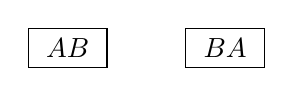
\begin{tikzpicture}[scale=1]
\draw (0,0.0) +(-.5,-.25) rectangle ++(.5,.25);
\draw (0,0.0) node{$A B$};x
\draw (2.0,0) +(-.5,-.25) rectangle ++(.5,.25);
\draw (2.0,0) node{$B A$};
\end{tikzpicture}
\end{figure}

We have two pairs of seats that can be satisfied completely with a single exchange. Since we cannot possibly make more than 2 couples happy with a single exchange, the optimal solution will contain as many of these as possible.  

\begin{lem} 
If a either of the seated couples in win-win exchanges are misaligned, it requires 2 swaps to make both pairs happy.
\end{lem}

\begin{proof}
Without loss of generality, we call the first, unaligned pair $A_1B_1$ and the second $A_2B_2$.  Since the first pair is unaligned, any exchange to pair it or its seatmate will necessarially not include $B_1$.  
\end{proof}

\begin{cor} \label{cor:winWinAsBlocks}
If a consecutive block of $N$ win-win pairs is misaligned, it requires $N$ more exchanges to satisfy all pairings than if they were all aligned.
\end{cor}

Win-win exchanges are 2 couples that can both be paired with a single exchange.  We would like to generalize this, calling win-win exchanges a two chain.  Three chains are three pairs that can all be satisfied with 2 exchanges like the example below:

\begin{figure}[H]
\centering
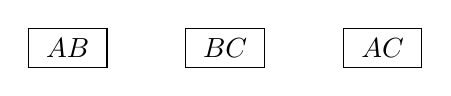
\begin{tikzpicture}[scale=1]
\draw (0,0.0) +(-.5,-.25) rectangle ++(.5,.25);
\draw (0,0.0) node{$A B$};x
\draw (2.0,0) +(-.5,-.25) rectangle ++(.5,.25);
\draw (2.0,0) node{$B C$};
\draw (4.0,0) +(-.5,-.25) rectangle ++(.5,.25);
\draw (4.0,0) node{$A C$};
\end{tikzpicture}
\end{figure}

This generalizes to $N$ chains, where chains are characterized by $N$ pairs that can all be satisfied with exactly $N-1$ swaps.

\subsection{Performance Ratio of Sweep Algorithm}

Our sweep algorithm ensures that we leave in place as many completed couples as possible. We do this because each completed couple we leave in place requires zero swaps, while setting them to be unaligned introduces new exchanges into our solution.  The ratio of unaligned exchanges to aligned exchanges is thus infinite, something to be avoided if we want a to bound the badness of a solution.

In its current incarnation, our algorithm ignores all $N$-chains.  Since each $N$-chain optimally requires $N-1$ swaps, failing to optimally align our couple seats will cost us at most $\frac{N}{N-1}$ times the optimal number of exchanges.  That is, our current algorithm is a 2 approximation.

\section{Conclusions}

We have introduced the novel problem of rearranging passengers on an airplane.  For even the special case of the airplane only having one row, we have shown in the general case of large families that this problem is NP complete.  The simple case of all passengers being in couples was solved optimally. For the more difficult case of all passengers being either alone or in couples, our algorithm was shown, first via simulations and then analytically, to be a 2 aproximation to optimal.

Our future work plans on analyzing heterogeneous family sizes larger than 2, and homogeneous small families as our hardness proof depended on arbitrarially large heteroeneous families. We would also like to analyze two dimensional planes with realistic seating arrangements, and families that nned not sit in one complete block, but where all family members has at least one familial neighbor.

Obviously, the optimization versions of all of these questions is also of interest.

\bibliographystyle{plain}
\bibliography{airplanePapers}{}

\end{document}
